\documentclass[10pt,a4paper]{scrartcl}
\usepackage[latin1]{inputenc}
\usepackage{amsmath}
\usepackage{amsfonts}
\usepackage{amssymb}
\usepackage{multicol, float}
\usepackage[hidelinks]{hyperref}
\usepackage[none]{hyphenat}
%\usepackage{setspace}
\usepackage{graphicx}
%\usepackage[export]{adjustbox}
\title{Research Journal Based On A. M. Turing, Computing Machinery and Intelligence}
\subtitle{COMP110 - Research Journal}
\author{1700522}
\begin{document}
	\maketitle
	%\begin{multicols}{2}
	\section{Introduction}
	In 1950 Alan Turing posed the question ``Can machines think?''\cite{turingComputing} a question that to this day has not truly been answered. Artificial Intelligence or AI research has a number of focuses exploring Turing's initial question utilising multiple methods. This journal will be looking into the use of AI in video games to create what Bridger calls a ``brain vs brain''\cite{BridgerFundamentalAI} scenario. It is important in the context of this journal to understand the difference between machine learning and deep learning as well as what the Turing Test is. 
	\section{The Imitation Game}
The Imitation Game is often referred to as the `Turing Test' and was set out by Alan Turing in Computing Machinery and Intelligence\cite{turingComputing}. The Imitation Game tests an AI to see if it can evolve and adapt to a conversation the same as a human would. The imitation game requires an AI to be able to work without perfect information, this is the only way the ``interrogator'' will not be able to tell if it is a person or computer. As it currently stands no AI has ever truly passed Imitation Game. This delves into the field of artificial human interaction as this is what the Turing Test is based on. While the Imitation Game tests if a human can be fooled by an AI is this the best place to focus our research? It is the position of this journal that Turing's ideas for AI were in fact flawed and the best focus for AI research is applying AI to problem solving as to best apply AI to benefit society.   
	\section{Machine Learning vs Deep Learning}
		In AI research one of the focuses is the training of these AI units to be able to reliably complete tasks and there are 2 main ways to do this, Machine Learning and Deep Learning.
		\subsection{What is Machine Learning?}
		Machine Learning can be defined as ``The capacity of a computer to learn from experience, i.e. to modify its processing on the basis of newly acquired information.'' according to the Oxford dictionary\cite{OxfordDictionary}. This means that machine learning works through the adapting to new information that is presented to it and that it can `learn' through completing the same task multiple times. This is how AIs learned to play checkers\cite{SamuelCheckers} and chess\cite{ShannonChess}. This research lead to the `Deep Blue' defeating the world chess champion\cite{DeepBlue}. 
		
		Machine Learning is split into 3 types of algorithms; Supervised learning, unsupervised learning and reinforcement learning. Supervised Learning algorithms can be described as ``The algorithm consist of a target / outcome variable (or dependent variable) which is to be predicted from a given set of predictors (independent variables). Using these set of variables, we generate a function that map inputs to desired outputs. The training process continues until the model achieves a desired level of accuracy on the training data.''\cite{EssentialMachineLearningAlgorithms}.
\begin{figure}[H]
	\begin{center}
	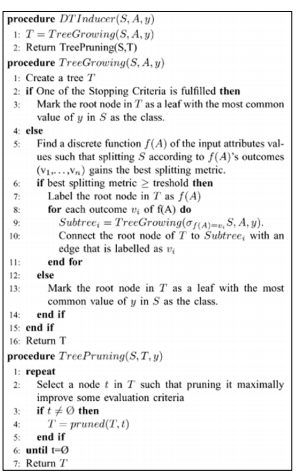
\includegraphics[width=0.5\textwidth] {pseudocodeDecisionTree.png}
	\caption{Pseudo code for Decision Tree \cite{MachineLearningAlgorithmsReview}}
	\label{DecisionTreePseudoCode}
	\end{center}
\end{figure}
Figure \ref{DecisionTreePseudoCode}	above shows the algorithm for a decision tree search, this is a type of supervised learning algorithm.	

		 Unsupervised Learning algorithms can be described as ``This algorithm, we do not have any target or outcome variable to predict / estimate.  It is used for clustering population in different groups, which is widely used for segmenting customers in different groups for specific intervention.''\cite{EssentialMachineLearningAlgorithms}.
\begin{figure}[H]
	\begin{center}
	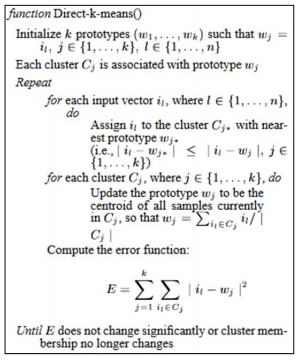
\includegraphics[width=0.5\textwidth] {pseudoCodeKCluster.png}
	\caption{Pseudo code for k-means clustering \cite{MachineLearningAlgorithmsReview}}
	\label{KMeansClusteringPseudoCode}
	\end{center}
\end{figure}		 

Figure \ref{KMeansClusteringPseudoCode} shows the algorithm for k-means clustering, this is a type of unsupervised learning algorithm.

		  Reinforcement Learning algorithms can be described as ``This algorithm, the machine is trained to make specific decisions. It works this way: the machine is exposed to an environment where it trains itself continually using trial and error. This machine learns from past experience and tries to capture the best possible knowledge to make accurate business decisions. ''\cite{EssentialMachineLearningAlgorithms}.
Temporal Difference Learning, (or TD learning) is a reinforcement learning algorithm that was used in 1995 by Tesauro to play backgammon \cite{TDGammon}. TD-Gammon was the attempt to make use of TD learning to play the game backgammon at a high level. The results of Tesauro's research showed promise for reinforcement learning which could then be applied to other AI research in later years. 

\begin{figure}[H]
	\begin{center}
		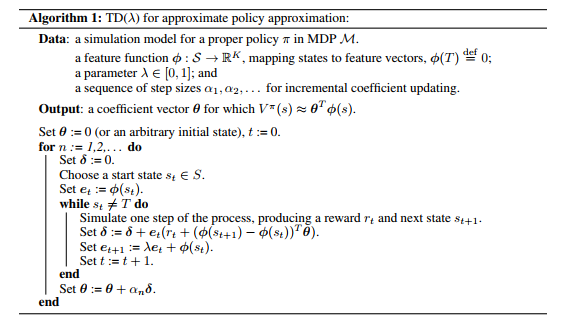
\includegraphics[width=1\textwidth] {pseudoCodeTDLearning.png}
		\caption{Pseudo code for temporal difference learning}
		\cite{TDLearningPseudoCode}
		\label{TemporalDifferenceLearningPseudoCode}
	\end{center}
\end{figure}
Figure \ref{TemporalDifferenceLearningPseudoCode} shows the algorithm for TD learning, this is a common refinforcement learning algorithm.
The Markov decision processes is a mathematical framework used within reinforcement learning. The MDP framework can be used in combination with dynamic programming to solve optimisation type problems the algorithm is as follows:
$$
(S, A, P.(\cdot,\cdot), R.(\cdot , \cdot), \gamma) 
$$
\begin{itemize}
	\item $S$ a potentially finite set of states
	\item $A$ a potentially finite set of actions ($A_{s}$ is the set of actions from the state of $s$)
	\item $P_{a}(s,s')$ is the probability that action $a$ in the state of $s$ at a given time will result in state $s'$ at the next time step
	\item$R_{a}(s,s')$ is the expected immediate reward from the change to $s'$ from $s$ as a direct result of $a$
	\item $\gamma \in [0,1] $ is the discount factor. This is the difference in future and present rewards.
\end{itemize}
The aim of MDP is to chose a policy ($\pi$) that maximises the function for rewards with the problem:
$$
\sum_{t=0}^{\infty} \gamma^{t}R_{a_{t}}(s_{t},s_{t}+1) 
$$
(where we choose $a_{t} = \pi(s_{t})$) \cite{MDP}
This is done through a combination of mathematical operations which allow the AI to reflect and build up its database through trial and error.

			\subsubsection{Monte Carlo Tree}
				In more recent years a method known as `Monte Carlo Tree Search' has evolved within machine learning, specifically within supervised learning. ``Monte Carlo Tree Search (MCTS) is a method for finding optimal decisions in a given domain by taking random samples in the decision space and building a search tree according to the results.''\cite{MonteCarloSurvey}. MCTS evaluates what the best option for the AI to take is and then takes it. Machine learning algorithms are used to allow the MCTS algorithm to calibrate itself so that it can correctly evaluate the options available in order to correctly select the optimal choice each time. MCTS has been applied to a number of games in order to test its effectiveness. MCTS has been applied to 2 games that this journal will explore Dou Di Zhu, (a popular Chinese card game)\cite{DouDiZhuMCTS} and Hearthstone, (an online collectable card game)\cite{HearthstoneMCTS}. In these examples Powley and Santos both explore how MCTS can be used in card games but with a very different set of rules and parameters. In his paper Santos defines MCTS as ``a de facto standard in game AI''\cite{HearthstoneMCTS} making this area of AI research incredibly relevant to the appliance of AI for problem solving rather than the mimicking of human interactions as Turing had in mind. This aligns with the views of this journal as it is for the application of AI for problem solving tasks.


		\subsection{What is Deep Learning?}
		Deep Learning is a method of training an AI as though it was a human brain, making use of artifical neurons to simulate human learning as described by Philbin\cite{CrashCourse}. Neural networks have recently. Deep Learning has been applied to research tasks across the world, one such example was in 2016 at Chungnam Nationality University in Korea, \cite{DeepLearningSmartwatches}. Lee's team discovered that they could use Deep Learning to work out how to reduce the distraction in smartwatch users. This application of artificial intelligence is very different to what has been seen so far in this journal. Most of the AIs this journal has looked at have been dedicated AIs, designed to to a single task well. Deep Learning AIs make use of artificial neural nets\cite{CrashCourse} and as such have the potential to be more like the Artificial Intelligence that Turing was referring to in 1950\cite{turingComputing}. This use of Deep Learning for simulating people in research was also used in Taipei at Tamkang University to assess the sentiment in reviews on Google Play\cite{GooglePlayTaipei}. This is what appears to be the use of Deep Learning, the simulation of human activity. This is further reinforced by Huawei making use of Deep Learning to aid in the design of their phones\cite{huawei}.


	\section{How does Machine Learning \& Deep Learning Compare?}
		Machine and Deep Learning algorithms appear to be designed for 2 very different tasks. A Machine Learning algorithm follows the more traditional path artificial intelligence has taken since the 1950's. As such Machine Learning has evolved to perform dedicated tasks such as play games like chess and Dou Di Zhu\cite{SamuelCheckers, ShannonChess, DeepBlue, DouDiZhuMCTS, HearthstoneMCTS}. Deep learning on the other hand seems like it is more likely to pass Turing's Imitation Game\cite{turingComputing} as the algorithms are designed to act more like human brains to the extent where they can be used for research \cite{CrashCourse, DeepLearningSmartwatches, GooglePlayTaipei, huawei}. Deep Learning makes use of incredibly expensive and complex hardware and as such is greatly under developed by comparison. It is the position of this journal that Machine Learning is greatly superior for dedicated tasks but Deep Learning is much closer to the general purpose AI that Turing was envisioning. Turing's envisionment of AI however in the author's did lack a question; Should we create an AI that can simulate humanity? As there is no knowing what a Strong Deep Learning AI would be capable of once technology reaches a point where it is possible. It is however the author's belief that a strong Deep Learning AI would beat the Imitation Game and pass the Turing Test.


	
	
	\newpage
	\bibliographystyle{ieeetran}
	\bibliography{references}{}
	
	%\end{multicols}
\end{document}